\subsection{Lab7: HackRF One}
%*********************
\begin{frame}{}

\pgfdeclareimage[width=\paperwidth,height=\paperheight]{bg}{imagenes/fondo_lab}
\setbeamertemplate{background}{\pgfuseimage{bg}}

\bfseries{\textrm{\LARGE Lab7\\ \Large HackRF One}}
\raggedright
\end{frame}
%*********************

\begin{frame}{HackRF One}

\pgfdeclareimage[width=\paperwidth,height=\paperheight]{bg}{imagenes/fondo3}
\setbeamertemplate{background}{\pgfuseimage{bg}}


HackRF One es un periférico SDR capaz de transmitir o recibir señales de radio desde 1 MHz hasta 6 GHz, fabricado por Great Scott Gadgets. Fue diseñado para facilitar el  desarrollo para las nuevas generaciones de tecnologías radio y sus correspondientes protocolos. Es un transceiver con capacidad de operación half-duplex .  Tiene una capacidad de muestreo de hasta 20 millones de muestras por segundo, pudiéndose alcanzar las 21,5 en función del tipo de controlador USB 2.0 HS que incluya el computador al que se conecta

\end{frame}
%-----------------------------------

\begin{frame}{Características}

\begin{center}
\vspace{-0.3cm}
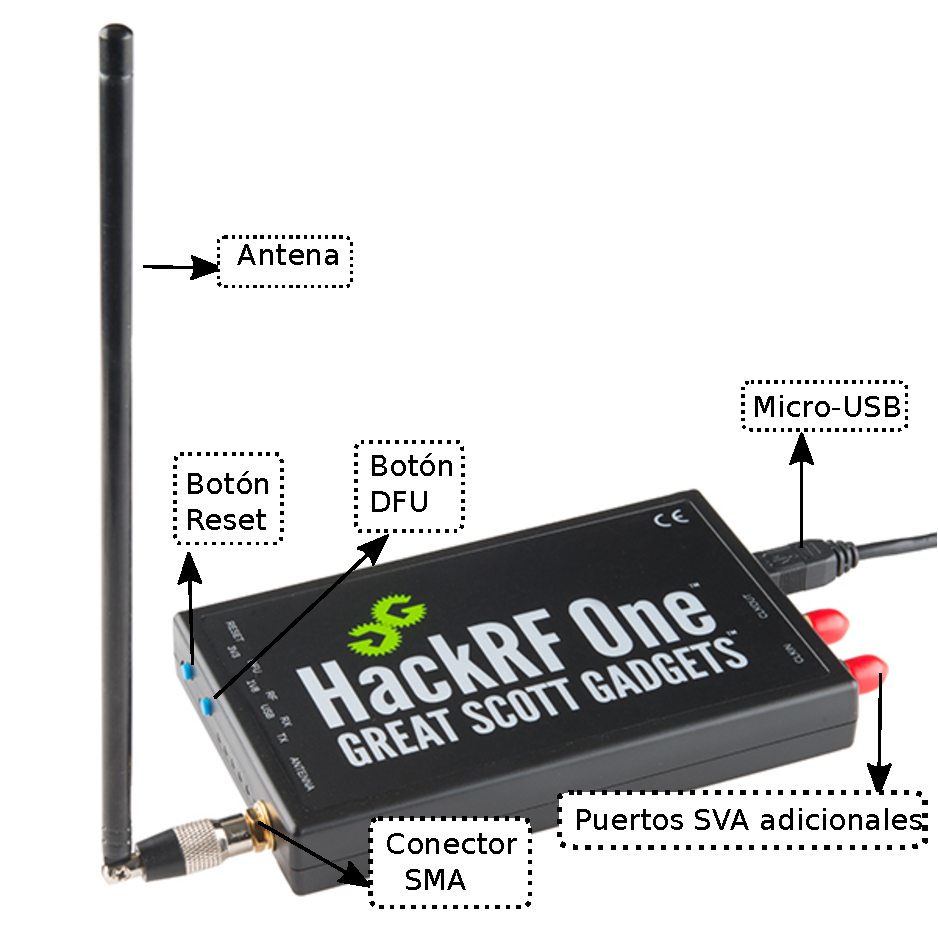
\includegraphics[width=.7\textwidth]{parte2/lab7/pdf/lab7_1.pdf}
\end{center}

\end{frame}
%-----------------------------------

\begin{frame}{Instalación de  herramientas de la HackRF One}

\begin{itemize}
    \item
    {Conecte el HackRF One a la computadora con el cable Micro-USB a USB. Confirme que los primeros tres  LEDs se iluminan para asegurar que el dispositivo esté funcionando.}
    \item
    {Las bibliotecas se pueden instalar con la siguiente órden en la terminal:
    
    \begin{block}{}
    \texttt{
    sudo apt-get install hackrf}
    \end{block}
    }
    \item
    {Después de la instalación, digite el comando "hackrf\_info" para verificar que el dispositivo HRF1 esté conectado.}
    
\end{itemize}
\end{frame}
%-----------------------------------

\begin{frame}{Instalación de  herramientas de la HackRF One}

\begin{itemize}
    \item
    {Estas son algunas herramientas utilizadas en HackRF One:
    \begin{itemize}
        \item  {\textit{hackrf\_info :} permite al usuario probar el dispositivo y mostrar la configuración.}
        \item  {\textit{hackrf\_max2837 :} permite al usuario controlar el chip max2837}
        \item  {\textit{hackrf\_spiflash :} permite al usuario configurar el Flash incorporado.}
        \item  {\textit{hackrf\_transfer :} permite al usuario recibir datos de RF y transmitir datos a RF.}
        \item  {\textit{hackrf\_si5351c :} permite al usuario controlar el chip si5351c.}
        \item  {\textit{hackrf\_cpldjtag :} permite al usuario configurar el CPLD integrado.}
    \end{itemize}
    }
\end{itemize}
\end{frame}
%-----------------------------------

\begin{frame}{Instalación de  herramientas de la HackRF One}

\begin{itemize}
    \item
    {Después de una instalación exitosa, la terminal debe responder con: \hspace{1pt} \ttfamily{found hackrf board}}
    \item
    {Si la terminal muestra que la HRF1 no está conectada, solucione los problemas verificando que los cables estén enchufados y se está suministrando potencia al dispositivo}
    
\end{itemize}
\end{frame}
%-----------------------------------

\begin{frame}{Actualización del firmware}

\begin{itemize}
    \item [Paso 1]
    {\textbf {Actualizar el firmware de SPI Flash }\\ Para actualizar el firmware en un HackRF One que funcione, use el programa hackrf\_spiflash:
    
    \begin{block}{}
    \texttt{
    hackrf\_spiflash -w hackrf\_one\_usb.bin}
    \end{block}
    
    Puede encontrar el firmware binario (hackrf\_one\_usb.bin) en el directorio firmware-bin del último paquete de versiones o puede compilar el suyo desde la fuente. Para Jawbreaker, use hackrf\_jawbreaker\_usb.bin. Si compila desde el origen, el archivo se llamará hackrf\_usb.bin. 
    }
    
\end{itemize}
\end{frame}
%-----------------------------------

\begin{frame}{Actualización del firmware}

\begin{itemize}
    \item [Paso 2]
    {\textbf {Actualizar el CPLD}\\ Para actualizar a la última imagen CPLD, primero actualice el firmware SPI flash, libhackrf y hackrf-tools. Entonces en la terminal se ingresa lo siguiente:
    
    \begin{block}{}
    \texttt{
    hackrf\_cpldjtag -x firmware / cpld / sgpio\_if / default.xsvf}
    \end{block}
    
    Después de unos segundos, tres LEDs deberían comenzar a parpadear. Esto indica que el CPLD se ha programado con éxito. Restablezca el dispositivo HackRF presionando el botón RESET o desenchufando y enchufando de nuevo.
    }
    
\end{itemize}
\end{frame}
%-----------------------------------

\begin{frame}{Instalación de paquetes para trabajar con GNU Radio: osmocom}

A continuación instalamos los paquetes de osmocom.

\begin{block}{}
    \texttt{
    \ \ \ git clone git://git.osmocom.org/gr-osmosdr}
\end{block}

Nos movemos dentro de la carpeta clonada:

\begin{block}{}
    \texttt
    {\ \ \ cd gr-osmosdr}
\end{block}


Creamos el directorio de construcción, nos movemos dentro y hacemos el cmake.

\begin{block}{}
  \texttt{
  \ \ \ mkdir build \&\& cd build
    \begin{itemize}
      \item[] cmake ../
    \end{itemize}}
\end{block}  
\end{frame}
%-----------------------------------

\begin{frame}{Instalación de paquetes para trabajar con GNU Radio: osmocom}
Construimos e instalamos.

\begin{block}{}
  \texttt{
  \ \ \ make
    \begin{itemize}
      \item[] sudo make install
      \item[]  sudo ldconfig
    \end{itemize}}
\end{block}  

\end{frame}
%-----------------------------------

\begin{frame}{Ejemplo mínimo}
    \begin{center}
    \vspace{-0.3cm}
    imagen
    %\includegraphics[width=\textwidth]{parte2/lab7/pdf/lab7_4.pdf}
    \end{center}
\end{frame}




